\subsection{Session 4, Exercise 7}

\lineparagraph{Exercise}

Create pushdown automata for the following languages.
\begin{enumerate}[a)]
    \item $L_a = \{a^ib^jc^k | i,j,k \geq{} 0\text{ and }i+j = k\}$
    \item $L_a = \{a^ib^jc^k | i,j,k \geq{} 0\text{ and }j+k = i\}$
    \item $L_a = \{a^ib^jc^k | i,j,k \geq{} 0\text{ and }i+k = j\}$
\end{enumerate}


\lineparagraph{Solution}

a)

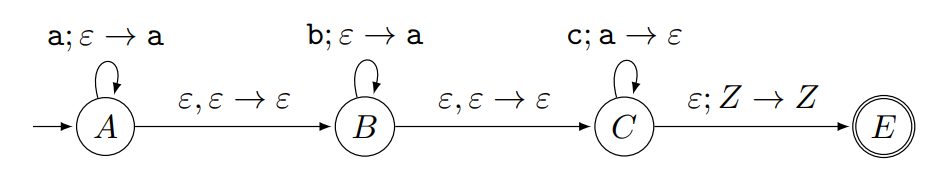
\includegraphics[width=\linewidth]{04/4_7_a.png}

TODO Proof

b)

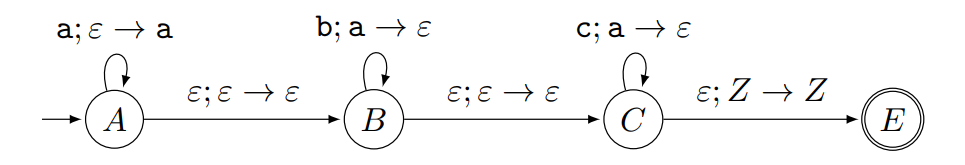
\includegraphics[width=\linewidth]{04/4_7_b.png}

TODO Proof

c)

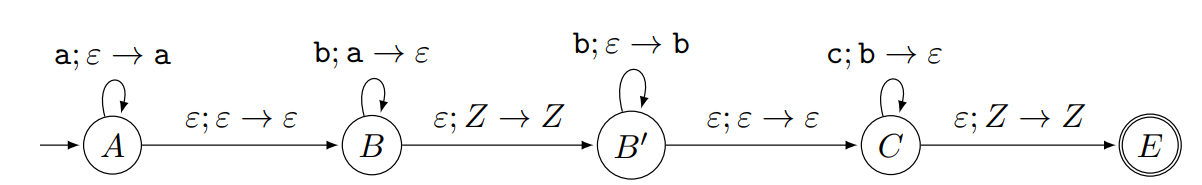
\includegraphics[width=\linewidth]{04/4_7_c.png}

TODO Proof

Note: c) is the tricky one, since we need the number of $a$'s plus the number of $c$'s to be equal to the number of $b$'s, but the $b$'s come in-between the $a$'s and the $c$'s. In this case we split the processing of $B$'s into two parts: in the first part we compare the number of $b$'s to the $a$'s that came before, while in the second part we store the number of $b$'s to be compared with the number of the upcoming $c$'s.

In this case we used non-determinism heavily, since the transition between $B$ and $B'$ must happen at the correct time for the calculation to work: one computational branch will time it correctly and that one can become an accepting branch (if everything else is correct with the word).